\newcommand{\uproman}[1]{\uppercase\expandafter{\romannumeral#1}}
\newcommand{\lowroman}[1]{\romannumeral#1\relax}
%% content.tex
%%

%% ==============================
\chapter{Prelude}
\label{ch:Introduction}
%% ==============================

\section{Abstract}

\vspace*{\fill}

Die Bildberechnung durch hardwareunterstützte Strahlenverfolgung und dazugehörige Techniken gewinnen gegenwärtig in der Echtzeitcomputergrafik an Bedeutung. 
Trotz dieser neuen Hardwareunterstützung entfällt nur wenig Rechenzeit auf die Berechnung eines
einzelnen Bildes. Einhergehend zu dieser kurzen Rechenzeit sind wiederrum weniger Pfade mit dementsprechend geringerer
Länge. Bereits frühere Arbeiten haben, um den so entstehenden Bildrauschen entgegenzuwirken,
die blue noise Fehlerverteilungen miteinbezogen und deren Bedeutung in der Steigerung der wahrnehmbaren Bildqualität hervorgehoben und verdeutlicht.
Diese Arbeit erläutert einen zeitlich stabilen Algorithmus aufgrund dieser Technik. Im Gegensatz zu vorhergehenden Ansätzen wollen wir direkt im Bildraum eine Fehlerumverteilung anwenden, um so eine entsprechend 
korrelierte Pixelfolge zu erhalten. All dies erreicht der Algorithmus ohne signifikanten Mehraufwand.
\vfill

\newpage

\section{Einleitung}
\vspace*{\fill}

Das \textit{q2vkpt}-Projekt(siehe \cite{Sch19}) zeigt beispielhaft den aktuellen Übergang in Echtzeitanwendungen, indem es in einem konventionellen Spiel die (teilweise) konventionelle Bilderzeugung 
mit neuen Technologien des \textit{Real-Time Raytracing} austauscht.

\begin{itemize}
    \item[Abschnitt \ref{ch:Content1:sec:Rasterisierung}] beschreibt die bisherige, konventionelle Herangehensweise und zeigt deren Limitierungen auf. Diese 
        Limitierungen führen uns zu einem Ansatz, der im 

    \item[Abschnitt \ref{ch:Content1:sec:Path Tracer}] besprochen wird. Hiermit lassen sich optische Phänomene, so z.B. Schatten, Spiegelungen \textit{korrekt} darstellen.
        Diese Technik wird durch die neue Hardwareunterstützung für Echtzeitanwendungen zugänglich, wenn auch mit deutlichen Leistungseinschränkungen.
        Aktuelle Entwicklungen wie in \cite{georgiev2016blue} haben sich in Bezug auf diese Technik mit \nameref{ch:Content1:sec:blue noise} dither masks beschäftigt
        und ihre Nützlichkeit in Steigerung der visuellen Qualität, bei geringer verfügbarer verbleibender Rechenzeit, gezeigt. Diese Ergebnisse motivieren den

    \item[Abschnitt \ref{ch:Content1:sec:blue noise}] über blue noise in welchem wir uns die Theorie aneignen und ihre Funktionsweise auf die Steigerung der 
        Bildqualität genau anschauen. Dabei liefert uns \cite{bluenoisechrisschied} eine blue noise Textur, welche wir im

    \item[Kapitel \ref{ch:Temporaler Algorithmus}]in einem temporalen Algorithmus, vorgestellt in \cite{hal02158423}, verwenden können. In zwei zusätzlichen Schritten, dem 
    \nameref{ch:Content2:sec:Sorting} und \nameref{ch:Content2:sec:Retargeting}, lassen sich unsere Pixel im Bildraum so korrelieren, dass eine zeitlich stabile Fehlerverteilungen
    entsteht. Dabei machen wir uns die Erkenntnisse aus Abschnitt \ref{ch:Content1:sec:Quasi-Zufallsfolgen} zu nutze, um nur eine Textur zu nutzen ohne jedoch auf den Effekt von mehreren 
    durchwechselnden Texturen verzichten zu müssen. Neben der vorberechneten blue noise Textur verwenden wir eine weitere \textit{Retarget}-Textur, welche wir erhalten, indem ein Optimierungsproblem 
    mit Hilfe der im  

    \item[Abschnitt \ref{ch:Content2:sec:Simulated Annealing}]vorgestellten Technik, dem Simulated Annealing, gelöst wird.   

\end{itemize}
 


\vfill
%% ==============
\chapter{Grundlagen}
\label{ch:Grundlagen}
%% ==============

%% ===========================
\section{Rasterisierung}
\label{ch:Content1:sec:Rasterisierung}
        Die Rasterisierung spielt in konventionellen Bilderzeugungsverfahren eine große Rolle. 
        Zu Beginn der Rasterisierung haben wir die Eckpunkte der bereits verarbeiteten, transformierten, projizierten Geometrie mit möglichen
        Beleuchtungsinformationen aus den vorherigen Berechnungen vorliegen (weiterführende Literatur \cite{akenine2018real}). 
        Mit Hilfe der Rasterisierung wird nun die Farbe jedes einzelnen Pixels bestimmt. Es ist also die Aufgabe der Rasterisierung herauszufinden, 
        welche Geometrie welchen Pixel zu welchen Anteil bedeckt und wie die Shading Informationen zur Farbgebung des Pixels beitragen. 
        Aufgrund dieser Vorgehensweise spricht man auch von einem objektbasierten Bilderzeugungsverfahren.

        \begin{figure}[H]
            \centering
            \includegraphics[width=\linewidth]{content/PathTracer/Bilder/Rasterisierung.pdf}
            \caption{Ablauf der Rasterisierung}
            \label{pic:Rasterisierungsablauf}
        \end{figure}

        Zuallererst befindet man sich im \nameref{pic:Rasterisierungsablauf} beim \textit{Triangle Setup}. Unbeeinflussbar vom Programmierer werden hier Daten berechnet, welche zur Pixeleinfärbung
        benötigt werden. So werden viele zuvor per Eckpunkt berechnete Werte interpoliert (Beleuchtung, Tiefe). Beim darauffolgenden \textit{Triangle Traversal} werden
        die wichtigen Fragmente erzeugt. Dieser Schritt bestimmt diejenigen Pixel, welche innerhalb des Dreiecks liegen und erzeugt darauf hin die Fragmente für dieses
        Dreieck anhand der zuvor berechneten/interpolierten per Dreieck Informationen. Als freiprogrammierbare Shadereinheit können im \textit{Fragment Shader}
        vom Programmierer weitere Berechnungen vorgenommen werden. Dazu zählt eine pro Pixel Beleuchtungsberechnung (Phong Shading).
        Im darauffolgenden Schritt wird mit dem Z-Buffer auf Sichtbarkeit geprüft. Die Ausgabe kann in mehrere verschiedene \textit{render targets}
        geschrieben und somit ein \textit{GBuffer} erzeugt werden. In einem ersten Schritt speichert man Informationen
        über das Material/Position vom Objekt in verschiedene \textit{render targets}. In einem zweiten Durchlauf kann man nun die Beleuchtung und einige andere 
        Effekte sehr effektiv berechnen.  
        Das abschließende nicht komplett freiprogrammierbare, aber hoch konfigurierbare \textit{Merging} hat eine besondere Aufgabe beim Abspeichern der Farbe für
        jeden Pixel im color Buffer. Zur Bestimmung der aktuellen Farbe wird nun auch das Problem der 
        Sichtbarkeit von Objekten angegangen. Zu den Z-Werten, welche wir als Tiefe beim Viewport Transform gespeichert haben, gibt
        es hier Zugang zum Depth/Z-Buffer. Dieser Z-Buffer speichert anfangs überall den Wert inf. Beim Durchlauf der Geometrie wird nun jeweils für jeden Pixel,
        der die Geometrie bedeckt der color und depth buffer wie folgt aktualisiert: Ist der verglichene Tiefenwert des vom Objekt erzeugten Fragment kleiner als der Wert
        im Tiefenbuffer für den betroffenen Pixel, so schreibt er diesen Tiefenwert in den Z-Buffer und auch der color Buffer mit der Fragmentfarbe aktualisiert.
        Falls nicht passiert nichts und das nächste Primitiv bzw. Fragment wird betrachtet (Szene ohne semitransparente Objekte!). Haben wir semitransparente Objekte, so 
        müssen wir zuerst die Szene wie beschrieben ohne diese Primitive zeichnen, alle semitransparenten Primitive nach ihrer Tiefe ordnen und in dieser Reihenfolge 
        zu dem zuvor gerenderten Bild hinzufügen. Damit haben wir auch unsere Projektion vollzogen, welche wir zuvor vorbereitet 
        haben(Weglassen der z-Komponente).\par 

        \subsection{Beschränktheit}
        \label{sec:Rasterisierung:Beschränktheit}

        Ihre bisherige weite Verbreitung hatte die Rasterisierung der Objektorientierung zu verdanken: massives paralleles Arbeiten, Ignorieren von (großen) leeren Bereichen und
        Ausnutzen von Cachekohärenzen gehören zu den Eigenschaften, welche die enorme effiziente, schnelle Abarbeitung bzw. (relativ) geringe aufzuwendende Rechenleistung begründen.
        Ihr großer Nachteil bzw. Beschränktheit liegt jedoch genau an dieser Objektorientierung. 
        Die Abbildung der Farbe eines Geometrie/Dreiecks auf einen Pixel simuliert
        den physikalischen Lichttransport nicht korrekt! Die physikalische Optik lehrt uns das Verfolgen von weiteren (sekundären) Strahlen abseits des Primärstrahls, der von 
        Sichtebene zum Objekt verläuft und durch die Rasterisierung im Gegensatz zu den Sekundärstrahlen abgedeckt wird. So können Effekte, welche diese Sekundärstrahlen involvieren, 
        entweder nicht oder nur (unzureichend befriedigend) dargestellt werden (z.B. Schatten, Spiegelungen). \par

        Die enormen Leistungsanforderungen von Technologien, welche diesen physikalisch korrekten Lichttransport möglich machen, haben Sie bisher für Echtzeitanwendungen ausgeschlossen.
        In heutigen modernen Grafikprogrammierschnittstellen (Vulkan, DirectX) jedoch befindet sich Raytracing-Funktionalität, welche auf Hardwareseite unterstützt wird.
        Diese Unterstützung erlaubt neuerdings erste image-ordered Bilderstellungen.  
        Aktuelle Bemühungen gehen nun daran Raytracing und Rasterisierung zu kombinieren. \cite{Barre-Brisebois2019} stellte
        mit dem Spiel \textit{PICA PICA} eine solche Rendering-Pipeline vor, welche mithilfe von Path Tracing arbeitet. Dabei wird der G-Buffer
        (Texturen die Position, Normalen, Belichtung eines Bildes speichern) noch über Rasterisierung berechnet. Direkten Schatten kann man 
        rastern oder durch das Verschießen von Strahlen bekommen. Diese Option verspricht eine Anpassungsfähigkeit der Pipeline nach Leistungsfähigkeit der Hardware. Ähnlich können nun
        Reflexionen, Global Illumination, Ambient Occlusion und Transmission durch Verschießen von Strahlen oder auf Compute Shader ausgeführt werden.(Wieder je nach 
        Hardwareleistung). Einzig direkte Beleuchtung sowie Post-Processing Effekte laufen nur über Compute-Shader. \par

        Wir wollen diesen Ansatz in dieser Arbeit aufnehmen. Berechnung des \textit{GBuffer}'s mit Hilfe von Rasterisierung und globale Beleuchtung durch 
        einen \nameref{ch:Content1:sec:Path Tracer} erreichen. Da trotz hardwarebeschleunigtes Strahlenverschießen unsere Anzahl an Strahlen beschränkt ist, 
        beschäftigen wir uns innerhalb dieser Arbeit mit einem \nameref{ch:Temporaler Algorithmus}, der die visuelle Qualität nicht durch Verschießen von mehr Strahlen, 
        sondern durch eine zeitlich stabile \nameref{ch:Content1:sec:blue noise} Fehlerverteilungen im Bildraum erreicht.
%% ===========================

%% ===========================
\newpage
\section{Path Tracer}
\label{ch:Content1:sec:Path Tracer}
\subsubsection{Funktionsweise}
Bei der Bilderzeugung, ausgehend von Szenen, welche viel Geometrie beinhalten bzw. bei Szenen 
die generelle BRDF's verwenden eignet sich das \ref{ch:Content1:sec:PathTracer}path tracing \cite{kajiya1986rendering}.
Das \ref{ch:Content1:sec:PathTracer}path tracing ist in Hinsicht der Beleuchtung komplett. Deshalb lässt sich damit
\textit{Global Illumination} erreichen. Das hier verwendete \ref{ch:Content1:sec:PathTracer}path tracing in 
\cite[eragae]{Benty18} verwendet eine klassische Umsetzung.\par

\begin{figure}[H]
    \centering
    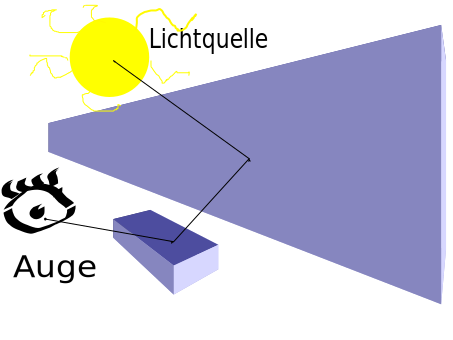
\includegraphics[width=0.7\linewidth]{content/PathTracer/Bilder/Grundkonzept_path_tracing.pdf}
    \label{pic::PathTracingGrundkonzept}
    \caption{Grundkonzept path tracer}
\end{figure}


Wie in \cite{marschner2009fundamentals} beschrieben wird ausgehend von der vollständigen Transportgleichung
\begin{equation}\label{eq:vollstaendige Transportgleichung}
    L_s(k_0) = L_e(k_0) + \int_{all(k_i)}^{} \rho(k_i, k_0)*L_f(k_i)*cos(\theta_i)d\theta_i
\end{equation}
    
\begin{equation}\label{eq:kajiya}
        I(x,{x}^{'}) = g(x,{x}^{'}) * \biggl[\epsilon(x,{x}^{'}) + 
                        \int_{S}^{} \rho(x,{x}^{'},{x}^{''})
                        I({x}^{'},{x}^{''}d{x}^{''})\biggr] 
\end{equation}
Sie beschreibt den Energietransport \textit{I} von einem Punkt ${x}^{'}$
zu einem Punkt x. Dabei ist ein maßgebender Faktor der Geometrieterm \textit{g},
der die relative Lage der beiden Punkte zueinander im Raum beschreibt.
Ein weiterer Faktor ist die Abstrahlung \textit{$\epsilon$} von ${x}^{'}$ nach x. 
Beeinflusst wird der Energiefluss auch durch
die bidirektionale Verteilungsfunktion \textit{$\rho$}, welche Aufschluss über
das einfallende Licht von einem Punkt ${x}^{''}$ über ${x}^{'}$ zu x gibt.\par
Die Schlussfolgerung aus dieser Gleichung \ref{eq:kajiya} ist: Die transportierte
Intensität von einem Licht zu einem Anderen ist die Summe des ausgestrahlten Lichts 
und das ausgestrahlte Licht zu x von allen anderen Oberflächen.


\subsubsection{Monte-Carlo-Integration}
Mit der Monte Carlo Integration approximieren wir die Rendergleichung.\par 
Bei gegebener Funktion \textit{f }:\textit{ S}$\rightarrow \mathbb{R}$ und der 
Wahrscheinlichkeitsdichtefunktion $x \sim p$
\cite{KK02}
\label{pic:MonteCarloIntegration}
\begin{equation}\label{eq:montcarlo}
    \int_{x\in S} g(x) d\mu \simeq \frac{1}{N}*\sum_{i=1}^{N}\frac{g(x_i)}{p(x_i)}
\end{equation}

\begin{figure}[H]\label{pic:WeissesRauschenTracer}
    \centering
    \begin{minipage}[t]{0.45\linewidth}
        \centering
        \includegraphics[width=\linewidth]{content/PathTracer/Bilder/WeissesRauschenSzene.png}
        \caption{Szene mit Weißem Rauschen}
    \end{minipage}
    \hfill
    \begin{minipage}[t]{0.45\linewidth}
        \centering
        \includegraphics[width=\linewidth]{content/PathTracer/Bilder/FFT_Ausschnitt2.png}
        \caption{FFT des Ausschnitts}
    \end{minipage}
\end{figure}




%% ===========================


%% ===========================
\newpage
\section{Blue Noise}
\label{ch:Content1:sec:blue noise}
\subsection{Eigenschaften}

Wie in \cite{Pet17} vorgestellt, macht man sich die Eigenschaften einer
blue noise Textur zu Nutze. Dabei werden im Folgenden, die dort bereit 
gestellten blue noise verteilten Texturen verwendet, welche anhand des in
\cite{ulichney1993void} vorgestellten Algorithmus erstellt wurden.
Die korrespondierenden Spektren werden mit Hilfe von \cite{FFTProgWeb} erstellt.

\subsubsection{Uniformität}
Die Uniformität(lat. \textit{uniformitas}-Einförmigkeit) garantiert uns 
wie in \cite{3288} eine gleichverteilte Wahrscheinlichkeitsdichtefunktion
mit zugehöriger gleichverteilter Wahrscheinlichkeitsfunktion. In \cite{Pet17}
sieht sie wie folgt aus: 

\begin{equation}\label{eq:uniformität}
    P(n \leq p) = p
\end{equation}

\subsubsection{Niedrige Frequenzen}
Niedrige Frequenzen sind in einer blue noise sehr wenig bis gar nicht 
vertreten. Dies ist an dem schwarzen Ring innerhalb der Fouriertransformierten
zu erkennen\ref{pic:blueNoiseFFT}.

\begin{figure}[H]\label{pic:blueNoiseFFT}
    \centering
    \begin{minipage}[t]{0.45\linewidth}
        \centering
        \includegraphics[width=\linewidth]{content/BlueNoise/Bilder/LDR_LLL1_0.png}
        \caption{$512^{2}$ blue noise Textur}
    \end{minipage}
    \hfill
    \begin{minipage}[t]{0.45\linewidth}
        \centering
        \includegraphics[width=\linewidth]{content/BlueNoise/Bilder/FFT_LDR_LLL1_0.png}
        \caption{Fourier Spektrum $512^{2}$ blue noise Textur}
    \end{minipage}
\end{figure}

\begin{figure}[H]\label{pic:bayerPatternFFT}
    \centering
    \begin{minipage}[t]{0.45\linewidth}
        \centering
        \includegraphics[width=\linewidth]{content/BlueNoise/Bilder/BayerMatrix.png}
        \caption{$512^{2}$ bayer pattern Textur}
    \end{minipage}
    \hfill
    \begin{minipage}[t]{0.45\linewidth}
        \centering
        \includegraphics[width=\linewidth]{content/BlueNoise/Bilder/FFT_BayerMatrix.png}
        \caption{Fourier Spektrum $512^{2}$ bayer pattern Textur}
    \end{minipage}
\end{figure}

\begin{figure}[H]\label{pic:tiledBlueNoiseFFT}
    \centering
    \begin{minipage}[t]{0.45\linewidth}
        \centering
        \includegraphics[width=\linewidth]{content/BlueNoise/Bilder/BlueNoise64Tiled.png}
        \caption{$512^{2}$ bayer pattern Textur}
    \end{minipage}
    \hfill
    \begin{minipage}[t]{0.45\linewidth}
        \centering
        \includegraphics[width=\linewidth]{content/BlueNoise/Bilder/FFT_BlueNoise64Tiled.png}
        \caption{Fourier Spektrum $512^{2}$ bayer pattern Textur}
    \end{minipage}
\end{figure}

\subsubsection{Isotropie}
Die Isotropie(altgr. \textit{isos}-gleich und \textit{tropos}-Richtung)
einer blue noise Textur wird ausgenutzt. Dabei haben wir in allen
Dimensionen (in dieser Arbeit werden Texturen mit zwei benutzt) 
die Unabhängigkeit einer Eigenschaft. 


\subsubsection{Kachelung}
Eine weitere nützliche Eigenschaft der blue noise Verteilung ist die 
Möglichkeit der Kachelung. 
%% ===========================


%% ===========================
\newpage
\section{Quasi-Zufallsfolgen}
\label{ch:Content1:sec:Quasi-Zufallsfolgen}
Sobol \cite{owen1998scrambling} \cite{heitz:hal-02150657} \cite{quasirandomsequencesbyRoberts}
\todo{find appropriate information and add it}

%% ===========================


%% ===========================
\newpage
\section{Simulated Annealing}
\label{ch:Content2:sec:Simulated Annealing}
Im vorherigen Kapitel, dem Retargeting Schritt \nameref{ch:Content2:sec:Retargeting},
wird eine vorberechnete Retargeting-Textur verwendet. Diese speichert eine
Permutation, die unsere blue noise Textur vom frame t in eine
blue noise Textur vom frame t+1 umwandelt. Diese Permutation wird 
dann auf die Startwerte angewandt bevor das nächste frame t+1 gerendert wird.
Dadurch werden die blue noise Umverteilung der Sorting Phase \nameref{ch:Content2:sec:Sorting}
akkumuliert und die optische Aufwertung erst richtig sichtbar.
Die retarget Textur wird mit Hilfe von \textbf{simulated annealing} 
\cite{hal02158423} berechnet. Wir wollen somit eine approximativ 
optimale Lösung finden: Permutiere Pixel der blue noise Textur von 
frame t bis Sie sehr ähnlich verteilt sind wie die Pixel der blue noise
Textur von frame t+1. Dabei ist die Lokalität der Vertauschungen, 
welche wir bereits in der Sorting Phase\nameref{ch:Content2:sec:Sorting}
verwendet haben, wichtig.

Die Funktion nach der optimiert wird ist an die Formel aus\cite{georgiev2016blue} angelehnt.
\begin{equation}\label{eq:pixel energy function}
    E(M) = \sum_{p \neq q}E(p,q) = 
           \sum_{p \neq q} \mathrm{e}^{-\frac{\Vert{p_{i}-q_{i}}\Vert^{2}}{\sigma_{i}^{2}} -
           \frac{\Vert{p_{s}-q_{s}}\Vert^{d/2}}{\sigma_{s}^{2}}}
\end{equation}
Wähle nach \cite{ulichney1993void} $\sigma_{i} = 2.1$ und $\sigma_{s} = 1$ 
Zu den Pixeln p,q beschreibt $p_{i}$ und $q_{i}$ ihre jeweiligen Koordinaten.
Und $p_{s}$ und $q_{s}$ sind ihre d-dimensionalen Samplewerte.


\begin{algorithm}[H]
    \caption{\textbf{Simulated Annealing} finde sehr gute Lösung}
    \begin{algorithmic}[1]
        \State initialisiere Startzustand $s=s_{0}$
        \For{i=1...maxSteps}
        \State //Radius für Nachbarschaftssuche ist auf 6 festgesetzt
        \State $s_{neu}\leftarrow$Nachbarzustand(s)
        \If{P(Energie(s), Energie($s_{new}$))$\ge$ random(0,1)} 
        \State s = $s_{new}$
        \EndIf
        \EndFor
        \State return Endzustand s;
    \end{algorithmic}
    \label{alg:retargeting}
\end{algorithm}

Als Startzustand $s_{0}$ definieren wir eine Permutation, die alle 
Elemente auf sich selbst abbildet.
Um von einem Zustand s zu einem neuem Zustand $s_{new}$ zu kommen,
definieren wir eine Nachbarschaftsfunktion \textit{Nachbarzustand()}. 
Diese kann zwei Elemente genau dann vertauschen, wenn Sie in einem 
gegenseitigen Radius r = 6 erreichbar sind. Dabei vertauschen wir
in jedem Schritt ein Pixelpaar. 
Die Wahrscheinlichkeitsfunktion zur neuen Zustandsannahme
P(Energie(s), Energie($s_{new}$)) beschreibt, ob wir den neu
gewählten Zustand $s_{new}$ übernehmen. Dabei wird klassischerweise die
Akzeptanz von Zuständen mit höherer Energie immer kleiner.(bzw. die 
Toleranz gegenüber größeren Fehlern im Bezug zur Zeit). Die allgemeine Akzeptanz von 
Zuständen mit höherer Energie ist dabei von fundamentaler Bedeutung.
Somit verlassen wir möglicherweiße nur lokale Maxima.
Die zu minimierende Energiefunktion E\nameref{eq:pixel energy function} betrachtet
dabei zwei 

\begin{figure}[H]\label{pic:Retargeting}
    \centering
    \begin{minipage}[t]{0.45\linewidth}
        \centering
        \includegraphics[width=\linewidth]{content/simulatedAnnealing/Bilder/LDR_RGBA_64.png}
        \caption{Blue noise Textur 64x64}
    \end{minipage}
    \hfill
    \begin{minipage}[t]{0.45\linewidth}
        \centering
        \includegraphics[width=\linewidth]{content/simulatedAnnealing/Bilder/LDR_RGBA_64_retarget_texture.png}
        \caption{Permutation; gespeichert in R,G-Channel einer .png}
    \end{minipage}
\end{figure}


%% ===========================


%% content.tex
%%

%% ==============
\newpage
\chapter{Temporaler Algorithmus}
\label{ch:Temporaler Algorithmus}
In diesem Abschnitt wird auf den in \cite{hal02158423} vorgestellten, temporalen Algorithmus eingegangen.
Dieser besteht grundsätzlich aus dem \nameref{ch:Content2:sec:Sorting} sowie den 
\nameref{ch:Content2:sec:Retargeting}. Es sollte unbedingt beachtet werden, dass folgende
Annahmen getroffen wurden: Der Algorithmus arbeitet Blockweise auf den Pixeln und erwartet, dass benachbarte
Pixel innerhalb dieses Blockes den selben Wert haben. Da wir einen temporalen Algorithmus haben, soll diese Annahme 
auch über mehrere gerenderte Bilder hinweg gelten. Es sollte also beachtet werden, dass der Algorithmus z.B. nicht 
für Objektkanten oder ruckartige Bewegungen (der Kamera oder Objekte) ausgelegt ist.
\cite{heitz:hal-02150657}

\cite{quasirandomsequencesbyRoberts}
\todo{find the right place for this chapter}\label{code:golden_ratio}
\begin{lstlisting}[style=CStyle]
   float g = 1.32471795724474602596; //Plastische Zahl
   float a1 = 1.0/g;
   float a2 = 1.0/(g*g);
   x[n] = (0.5+a1*n) %1; //toroidally shifted
   y[n] = (0.5+a2*n) %1; //toroidally shifted
\end{lstlisting}
Die sogenannte Plastische Zahl in \ref{code:golden_ratio} ist die Lösung der
Gleichung \ref{eq:plasticnumber}
\begin{equation}\label{eq:cubic}
   x^{3} - x - 1 = 0
\end{equation}
Die Lösung dieser Gleichung lässt sich über die Padovan und Perrin Sequenz
definieren. Damit erhalten wir Plastische Zahl $\Phi$:

\begin{equation} \label{eq:plasticnumber}
   \Phi = \frac{(9 - \sqrt{69})^{1/3} + (9 + \sqrt{69})^{1/3}}
               {2^{1/3}3^{2/3}}
\end{equation}

\todo{add further information and references!!!}
\cite{vanderlaanplasticnumber}
\cite{wolframalphaPlastic}

%% ==============

%% ===========================
\newpage
\section{A Posteriori}
\label{ch:Content2:sec:a Posteriori}
Um das in Abschnitt \ref{subsec:dither sampling} vorgestellte \textit{Dither Sampling} zu realisieren
benutzen wir für den temporalen Algorithmus \ref{ch:Temporaler Algorithmus} diese im Folgenden vorgestellten
\glqq nachträglichen\grqq Annahmen \cite{hal02158423}. 
A Posteriori sind Sie in dem Sinne, als das wir die Annahmen szenenabhängig machen und Sie anhand 
von bereits erstellten Pixelwerten formulieren. 

\subsection{Theoretische Grundlage}

Im Kapitel \nameref{ch:Content1:sec:Path Tracer} haben wir gesehen, dass 
wir den Wert eines Pixels (i,j) klassischerweise mit einem zufälligen
Startwert durch eine Monte-Carlo Integration erhalten. Wir betrachten im
Folgenden eine (theoretische) Menge von allen möglichen Werten eines 
Pixels, welche durch alle möglichen Startwerte generiert wurde.
In Abbildung \ref{eq:Pixel Schätzung Wahrscheinlichkeitsdichtefunktion} ist die Wahrscheinlichkeitsdichtefunktion
$h_{ij}$ aufgetragen, als eine Funktion über alle möglichen Werte 
$I_{ij}$ eines Pixels (i,j).

\begin{equation}\label{eq:Pixel Schätzung Wahrscheinlichkeitsdichtefunktion}
    H_{ij}([I_{Anfang},I_{Ende}]) = \int_{I_{Anfang}}^{I_{Ende}} h_{ij} dI
\end{equation}

Verfolgt man beispielhaft die Werte eines Pixels über neun Bilder bei unseren \nameref{ch:Content1:sec:Path Tracer}, 
so ergibt es sich zur Anschauung wie folgt:

\begin{figure}[H]

    \begin{subfigure}{\textwidth}
        \centering \includegraphics[width=0.6\linewidth]{content/TemporalerAlg/Bilder/APosteriori/frame_t_whitenosie2.0.png} 
        \caption{Szenenausschnitt}
        \label{fig:szene_pixel_position_512x512}
    \end{subfigure}

    \begin{subfigure}{0.5\textwidth}
        \centering \includegraphics[width=0.6\linewidth]{content/TemporalerAlg/Bilder/APosteriori/pixel_512x512_strip.png} 
        \caption{Werte des Pixels an Position 512x512 im zeitlichen Verlauf (grüner Pfeil)}
        \label{fig:ausschnitt_pixelstrip}
    \end{subfigure}
    \begin{subfigure}{0.5\textwidth}
            \centering
            \def\svgwidth{\columnwidth}
            \import{content/TemporalerAlg/Bilder/APosteriori/}{histogram_of_estimates.pdf_tex}
            \caption{Histogram der Pixelschätzungen}
            \label{pic:histogramOfEstimates}
    \end{subfigure}
        \caption{Pixelwerte an Position 512x512(grüne Markierung) in aufeinanderfolgenden Zeitschritten}
        \label{fig:Pixelwerte}

\end{figure}

Betrachten wir die theoretische, praktisch nicht umsetzbare Menge aller möglichen Werte. 
Mit dieser Menge haben wir ein vollständiges Histogramm. Dies bedeutet wiederrum, dass das Erzeugen eines 
Pixelwertes nichts anderes bedeutet, als eine zufällige Wahl anhand der impliziten
Wahrscheinlichkeitsdichtefunktion. Wir können als einem zufälligen Anfangswert einen konkreten 
Pixelwert zuteilen und eine umkehrbare Funktion definieren \ref{eq:inverse Funktion}. 

Daraus lässt sich die Gleichbedeutung zweier Aussagen begründen:
Das Rendern des Pixels (i,j) und das Wählen eines Pixelswertes $I_{ij}$
von unser zuvor formulierten Wahrscheinlichkeitsdichtefunktion $h_{ij}$.

\begin{equation}\label{eq:inverse Funktion}
    I_{ij} = H_{ij}^{-1}(x), x \in [0,1]
\end{equation}

\par

\textbf{Fazit}: Falls $x \in d_{ij}$, wobei d eine korrelierte Zahlenfolge, die einer 
\nameref{ch:Content1:sec:blue noise} Verteilung entspricht, folgt aus der bijektiven
Natur der Gleichung \ref{eq:inverse Funktion} eine \nameref{ch:Content1:sec:blue noise} 
Fehlerverteilungen im Bildraum. 

Anmerkung: Das Dies nur theoretisch möglich und gerade für Echtzeitanwendungen nicht umsetzbar ist, 
folgt eine praktikable Formulierung!

\subsection{Praktische Durchführung}

Die Berechnung des vollständigen Histogramms ist für eine Echtzeitanwendung
zu kostenintensiv. Stattdessen könnte man auch die dadurch beanspruchte 
Rechenleistung auf z.B mehrere Samples pro Pixel verteilen und dadurch eine 
Steigerung der Bildqualität erreichen!
Stattdessen werden wir in dem temporalen Algorithmus (siehe \cite{hal02158423})
das Histogramm mit dem vorherigen Bild approximieren. 
Die Approximation des Histogramms erfolgt dadurch mit dem $Frame_{t}$ 
für $Frame_{t+1}$. Daher ist eine getroffene Annahme, um die gute Funktionalität des 
Algorithmus zu garantieren, eine nicht zu schnelle Bewegung der Kamera.
Außerdem werden für das Histogramm eines Pixels seine umliegenden benachbarten Pixel gewählt.
Daher ist eine weitere getroffene Annahme, um die gute Funktionalität des 
Algorithmus zu garantieren, eine möglichst homogene Fläche. 
Offensichtliche Konsequenzen dieser blockweisen Verarbeitung sind schlechte blue noise 
Fehlerverteilungen im Bildraum bei sich stark ändernden Bildausschnitten
(so z.B. bei Objektkanten), da dort die Annahme, dass eine ähnliche Oberfläche
zur Farbgebung beiträgt verletzt wird.

\begin{figure}[H]
    \centering
    \begin{subfigure}[b]{0.4\textwidth}
        \centering \includegraphics[interpolate=false, width=\linewidth]{content/TemporalerAlg/Bilder/APosteriori/homogener_ausschnitt_blocksize.png}
        \caption{homogener Pixelblock}
        \label{fig:homogener Pixelblock}
    \end{subfigure}
    \begin{subfigure}[b]{0.4\textwidth}
        \centering \includegraphics[interpolate=false,width=\linewidth]{content/TemporalerAlg/Bilder/APosteriori/inhomogener_ausschnitt_blocksize.png}
        \caption{inhomogener Pixelblock}
        \label{fig:Inhomogener Pixelblock}
    \end{subfigure}

    \caption{Pixelblöcke bei (in-)homogenen Flächen}\label{fig:Pixelblöcke}
\end{figure}

In Abbildung \ref{fig:Inhomogener Pixelblock} sind die benachbarten Pixel eine gute 
Approximation des jeweiligen Pixels, wohingegen in Abbildung \ref{fig:homogener Pixelblock}
die benachbarten Pixel dies nicht sind.
%% ===========================



%% ===========================
\newpage
\section{Sorting}
\label{ch:Content2:sec:Sorting}
In diesem Schritt wollen wir nun die Untersuchungen aus 
\ref{ch:Content2:sec:APosteriori} durchführen. Nach dem Rendern eines
Frames t(vor dem Rendern von Frame t+1) approximieren wir das Histogramm
der Pixelwerte anhand der Pixelwerte von Frame t.
\cite{hal02158423}
\begin{algorithm}[H]
    \caption{\textbf{Sortier Schritt t} nach dem Rendern von Frame t
    und vor dem Rendern von Frame t+1}
    \begin{algorithmic}[1]
        \STATE pixel \textbf{consists of} value,index;
        \STATE List framePixelsIntensities, noiseIntensities;
        \STATE $assert(sizeof(framePixelsIntensities)==BLOCKSIZE)$;
        \STATE $assert(sizeof(noiseIntensities)==BLOCKSIZE)$;
        \STATE List L $\leftarrow$ pixels of frame t in block;
        \STATE \hfill
        \STATE //init lists
        \STATE initList(framePixelsIntensities, pixelIntensity(L);
        \STATE $blueNoise_{t}$ = calcCorrectOffset(incomingbluenoisetexture);
        \STATE initList(noiseIntensities, pixelIntensity($blueNoise_{t}$));
        \STATE \hfill
        \STATE //sort the two lists by means of intensities
        \STATE sort(framePixelsIntensities);
        \STATE Sort(noiseIntensities);
        \STATE \hfill
        \STATE //now we reorder our seeds hence the sorted lists
        \FORALL{$i = 1 .. BLOCKSIZE$}
        \STATE $sortedSeeds(noiseIntensities.getIndex(i)) = incomingSeeds(framePixelIntensities.getIndex(i))$;
        \ENDFOR
    \end{algorithmic}
    \label{alg:Sortier}
\end{algorithm}
%% ===========================



%% ===========================
\newpage
\section{Retargeting}
\label{ch:Content2:sec:Retargeting}
\cite{hal02158423}

Zu Grunde liegender Sinn dieses Schrittes: Vertauschen der Anfangswerte, die 
verteilt sind wie $BlueNoise_{t}$, sodass Sie verteilt sind wie die 
$BlueNoise_{t+1}$. Aufgrund dessen haben wir eine Aufsummierung der
blue noise Fehlerverteilungen über viele Frames.

\begin{algorithm}[H]
    \caption{\textbf{Retargeting Schritt} t Vor Rendern Frame t+1 nach Sortier Schritt}
    \begin{algorithmic}[1]
        \State //permutation indices from precomputed texture
        \State $retaget_{t}$ = retargettexure[calcCorrectOffset(incomingbluenoisetexture)];
        \State List<PixelPermutation> L = $retaget_{t}$
        \For{i = 1 .. numberOfPixelsPerBlock}
        \State $retargetedSeeds(L.getNewIndices()) = incomingSeeds(L.getOldIndices());$
        \EndFor
    \end{algorithmic}
    \label{alg:retargeting}
\end{algorithm}

%% ===========================

%% ===========================
\newpage
\section{Temporaler Ansatz}
\label{ch:Content2:sec:Temporaler Ansatz}
Das Problem der globalen Beleuchtung durch physikalisch basierter Monte-Carlo Integration und gleichzeitiges Erreichen der 
Echtzeitanforderung von 30$\frac{Bilder}{s}$ ist ein bekanntes Problem. Dazugehörige bekannte Lösungsansätze 
ziehen bereits temporale Lösungsansätze z.B. temporales Akkumulieren \cite{schied2017spatiotemporal} in Betracht. 
\par 

Eine klassisches Formulierung \cite{UE4TAA} haben wir beispielhaft wie im Folgenden angewandt:

\begin{algorithm}[H]
    \caption{Beispielhafte Akkumulation}
    \begin{algorithmic}[1]
        \State Texture2D current\_frame;
        \State RWTexture2D accumulation\_buffer;
        \State float4 current\_color = current\_frame[pixel\_pos];
        \State float4 prev\_color = accumulation\_buffer[pixel\_pos];
        \State accumulation\_buffer[pixel\_pos] = 
        \State (frame\_count * prev\_color + current\_color) / (frame\_count + 1);
    \end{algorithmic}
    \label{alg:TemporalAccumulation}
\end{algorithm}

Diese klassische Formulierung, verletzt unsere Annahme für die Quantilfunktion \ref{eq:inverse Funktion}
in den \nameref{ch:Content2:sec:a Posteriori}-Bedingungen des zugrundeliegenden Algorithmus 
\ref{ch:Temporaler Algorithmus}. Denn durch diese Akkumulation bestimmt nicht mehr allein der 
Anfangswert die Pixelfarbe!
\par 

\begin{figure}[H]
    
    \label{subsec:Temporales Projezieren}
\end{figure}
Um die a Posteriori Annahmen anwenden zu können und die Vorbedingungen der Quantilfunktion \ref{eq:inverse Funktion}
für unseren Algorithmus zu erfüllen brauchen wir eine erneute Permutation! Denn durch die Permutation haben wir wieder garantiert, 
dass je ein Anfangswert $x \in [0,1]$ auf je ein Pixelfarbwert abbgebildet wird. Wir nehmen die Idee zur Verbesserung der Zeitkohärenz
aus \cite[S.9/10]{hal02158423} auf. Da unser Algorithmus davon ausgeht, dass zwei aufeinanderfolgende Bilder gleiche Pixelwerte 
besitzen, erhoffen wir uns durch eine temporale Projektion ein Verbesserung bei der \nameref{ch:Content1:sec:blue noise} Verteilung 
falls sich z.B. durch Kamerabewegung die Farbgebung der Pixel zwischen Ihnen ändert. Die temporale Projektion, welche wir hier 
anwenden, baut auf aktuelle verbreitete Techniken des TAA auf \cite{INSIDETAA}.

\begin{figure}[H]
        \centering
        \includegraphics[width=\linewidth]{content/TemporalerAlg/Bilder/Reprojection/TemporalReprojectPrincipal.png}
        \caption{Übersicht Temporal Reprojection}
        \label{pic:Uebersicht_Temporal_Reprojection}
\end{figure}

Wir benutzen die berechneten Tiefenwerte aus dem GBuffer (siehe auch unserer \nameref{pic:Render Graph}) und die jeweiligen 
View-Projektion-Matrizen der Kameras, um herauszufinden welche Koordinaten der jeweilige Anfangswert von Bild t im Bild t+1 
haben würde aufgrund der Drehung.
\par 


%% ===========================

%% ===========================
\newpage
\section{Rechenaufwand und Speicherbedarf}
\label{ch:Content2:sec:Rechenaufwand}
Da unsere Ressourcen beschränkt sind und trotz Hardwarebeschleunigung immer noch viel Rechenzeit eines Frames auf die globale Beleuchtung entfällt,
ist es von Bedeutung, dass unser temporaler Algorithmus keinen signifikanten zusätzlichen Aufwand schafft.
Mit einem Großteil der Rechenzeit, der auf die Berechnung des GBuffers und der globalen Beleuchtung fällt sind wir hingegen 
mit den Schritten Sorting und Retargeting (+ temporal Reprojection) sowohl auf  CPU als auf GPU Seite im niedrigen Prozentbereich.
Dabei wurde hier eine Blockgröße (siehe Abschnitt \ref{subsec:Blockgröße}) von B = 64 verwendet. Bei einer kleineren Blockgröße von B = 16, welche 
bereits gute Ergebnisse liefert, reduziert sich der Aufwand auf ein Viertel. 
\par
\newcolumntype{Y}{>{\raggedleft\arraybackslash}X}% see tabularx
%\tcbset{enhanced,fonttitle=\bfseries\large,fontupper=\normalsize\sffamily,
%colback=yellow!10!white,colframe=red!50!black,colbacktitle=red!30!white,
%coltitle=black,center title}
\begin{figure}[H]
    \begin{tcolorbox}[title=Rechenaufwand]
        \begin{tcolorbox}[tabularx={X|Y|Y},title=Pipeline, colbacktitle=yellow!50!red, coltitle=white]
            \textbf{Stufen}                                     &  \textbf{Rechenzeit(ms/\%)} CPU & \textbf{Rechenzeit(ms/\%)} GPU \\\hline\hline
            \textbf{Gesamt}                                     &  29.55/100\%                    & 19.04/100\%\\\hline
            GBuffer                                             &  06.48/21.91\%                  & 01.30/6,83\%\\\hline
            Retargeting(+ optionale temporale Reprojektion)     &  01.12/3.8\%                    & 00.11/0.57\%\\\hline
            GGXGlobalIllumination                               &  21.20/71.74\%                  & 15.51/81,46\%\\\hline\hline
            Sorting(B=64)                                       &  00.75/2,53\%                   & 02.12/11,13\%\\\hline\hline
            \textbf{Nicht in Gesamt}                            &                                 &              \\\hline\hline
            Sorting(B=16)                                       &  00.75                          & 00.55        \\\hline\hline
        \end{tcolorbox}  
        \tcblower
        \begin{tcolorbox}[tabularx={X|Y|Y},title=Vorberechnungen, colbacktitle=yellow!50!red, coltitle=white]
            \textbf{Vorberechnung}        &  \textbf{Rechenzeit(m)}    &  \textbf{Fehler(raw/\%)}\\\hline\hline
            Retargeting                   &  17,07                     &  10714 $\approx$ 3.07\%\\\hline
            Retargeting                   &  35,36                     &  9444 $\approx$ 2,71\%\\\hline
            Temporale Projizieren         &  194,7                     &  $\approx$ 10000\\\hline\hline
        \end{tcolorbox}  
    \end{tcolorbox}
    \caption{Rechenzeiten die auf die einzelnen Stages fallen}
    \medskip
    \small
    * Hardware: AMD Ryzen 5 2600X, NVIDIA GeForce RTX 2060 SUPER\newline
    * Fehler: Anteil orientiert sich am Anfangsfehler von 348180 $\rightarrow$ Summe von pixelweise Differenz Blue Noise(t=0) und Blue Noise(t=1) 
\end{figure}

Um zu einem Ergebnis wie in Figur \ref{fig:annelaing animated}(siehe Abschnitt \nameref{ch:Content2:sec:Simulated Annealing}) zu kommen, braucht man $\approx17$ Minuten. 
Diese Berechnung liefert ein gutes Ergebnis bei akzeptablen Rechenaufwand. Für einen Fehler von (minimale Verbesserung) sind bereits $\approx17$ Minuten 
nötig.

%%%%%%%%%%%%%%%%%%%
%%%%% storage usage
%%%%%%%%%%%%%%%%%%%
Wie speichern unsere Anfangswerte in einer 1920x1080 32-Bit-Textur. Die \nameref{ch:Content1:sec:blue noise} Textur innerhalb des \nameref{ch:Content2:sec:Sorting} Schrittes 
ist eine 64x64 32-Bit Textur. Die Retarget-Textur benutzt eine 64x64 16-Bit Textur. Das temporale Projizieren benutzt 11 solcher Texturen.
\begin{figure}[H]
    \begin{tcolorbox}[tabularx={X|Y},title=Speicherbedarf, colbacktitle=red, coltitle=white]
        \textbf{Pipelinestage}  &  \textbf{Speicherbedarf/KB} \\\hline\hline
        Sorting                 &  16,1                     \\\hline
        Retargeting             &  12,1                    \\\hline
        Temporale Reprojektion  &  133,1                    \\\hline
        Anfangswerte(Seeds)     &  7920                     \\\hline\hline
        \textbf{Gesamt}         &  \textbf{8226,5}           \\\hline\hline                
    \end{tcolorbox}
    \caption{Speicherdarf}
\end{figure}


    
%% ===========================




